\section{Motivation}

Machine learning promises significant benefits for simplifying and
improving the construction of optimization heuristics by replacing
fragile and expensive hand-tuned heuristics with data-driven
statistical modeling. For this goal to be realized, we require machine
learning systems capable of reasoning about program semantics. Despite
tremendous gains in recent years, state-of-the-art approaches for
learning on code are not sufficiently powerful to replicate the
analysis tasks that are fundamental to compilers. The crux of the
problem lies in two central aspects of machine learning: input
representation and model algorithmic complexity.

\paragraph{(I) Input Representation}

To be processed by a Neural Network (NN), code inputs may be encoded
either directly from a source language, by way of AST analysis, or
using an IR. Examples of each abound in the
literature~\cite{Allamanis2017a,Chen2019,Wang2018}. One
state-of-the-art encoder, code2vec~\cite{Alon2018a}, uses AST paths to
embed programs. code2vec proves highly effective at software
engineering tasks such as algorithm classification, where the code was
written by humans. However, as shown in Figure \ref{subfig:code2vec},
the trained representation can put more weight on names rather than
code structure, where minute modifications completely change
classification outcome. There are many benefits to such a
representation, including smart pasting and automated
refactoring. However, when analyzing code for optimization, identifier
names are rarely of use, whereas structure and semantics should be the
primary consideration. For example, in choosing to represent code at
the AST level, the code2vec representation does not capture the data
or control relations between statements.

\begin{figure}[t]
  \centering
    \begin{subfigure}{.48\linewidth}
      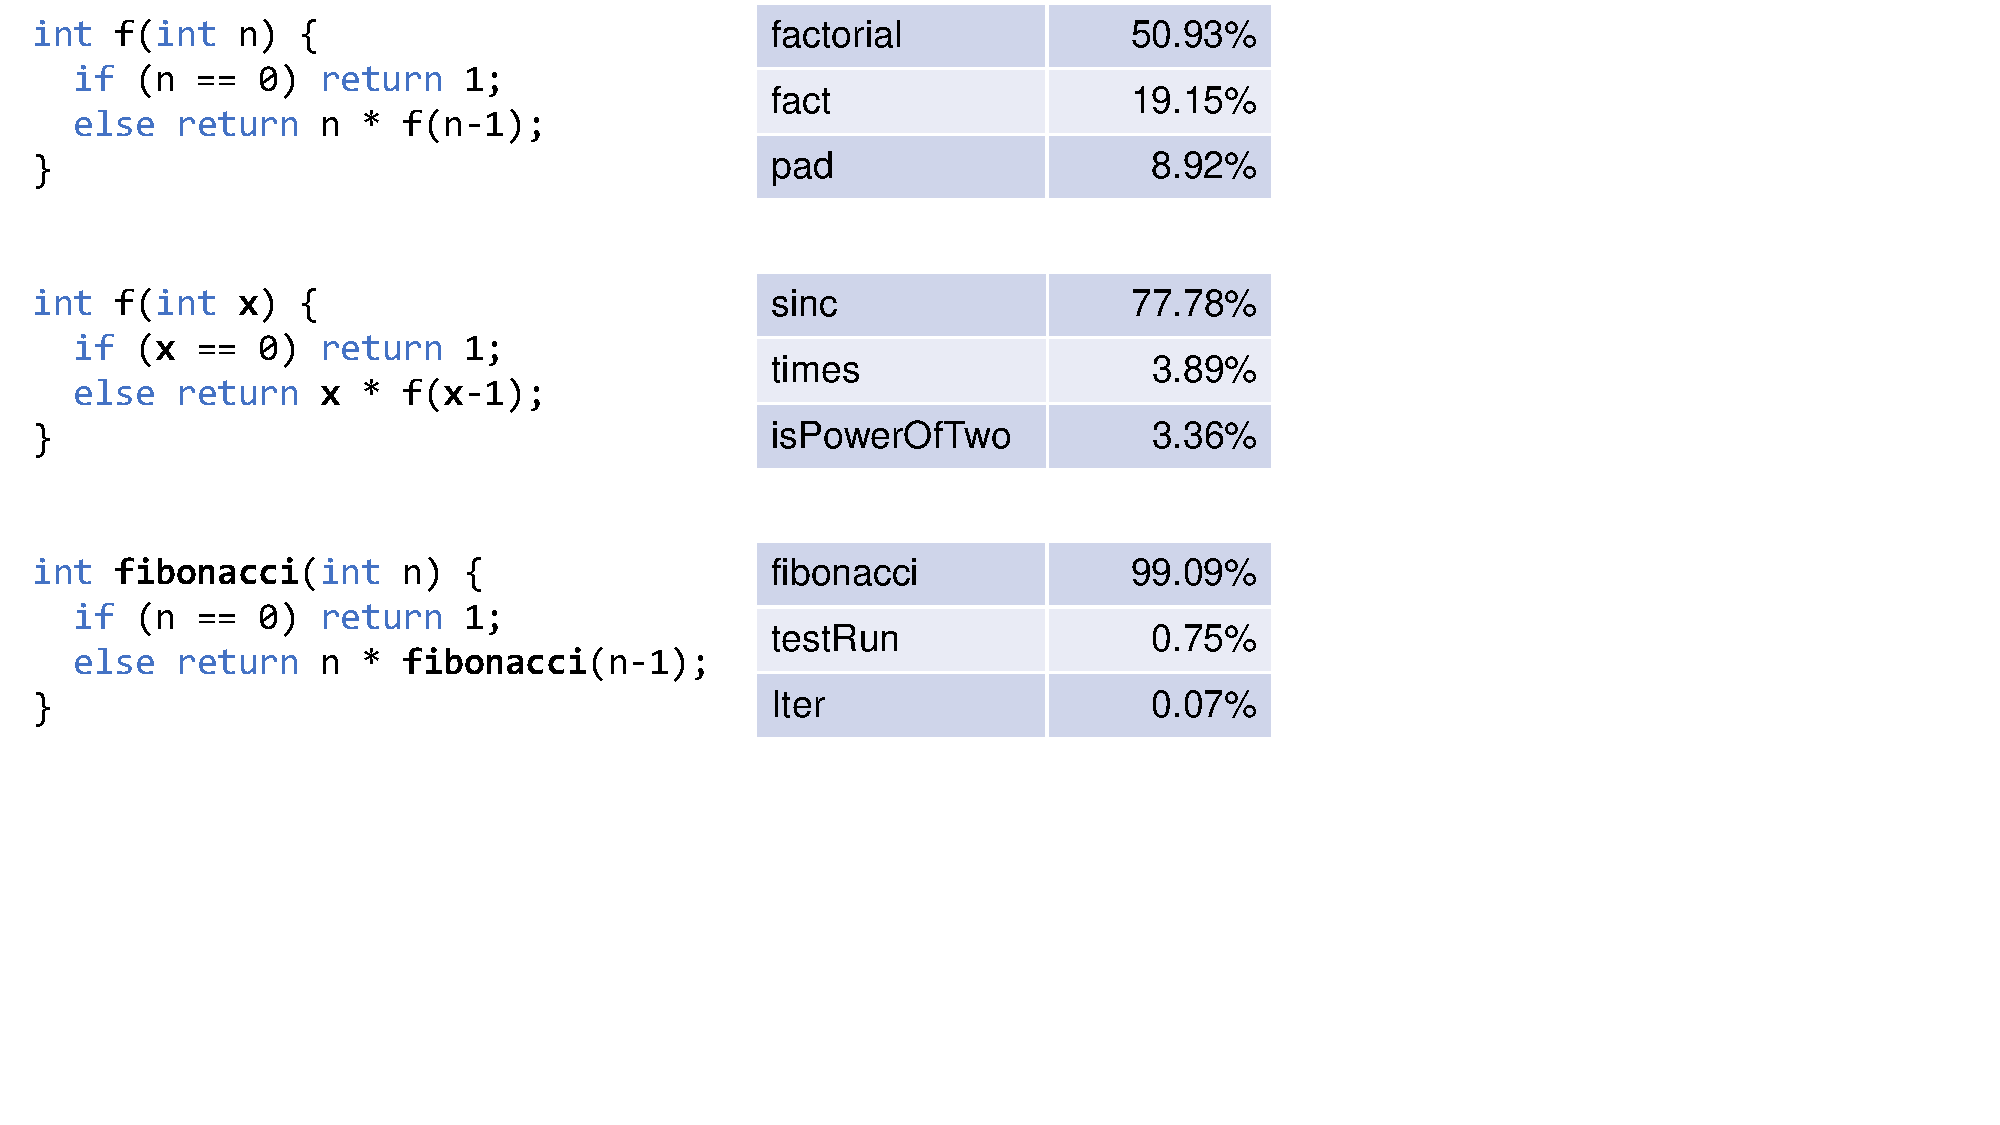
\includegraphics[width=\linewidth]{images/code2vec-transposed.pdf}
      \caption{code2vec~\cite{Alon2018a}.}
      \label{subfig:code2vec}
  \end{subfigure}
  \hfill
  \begin{subfigure}{.29\linewidth}
    \vspace{2.5em}
      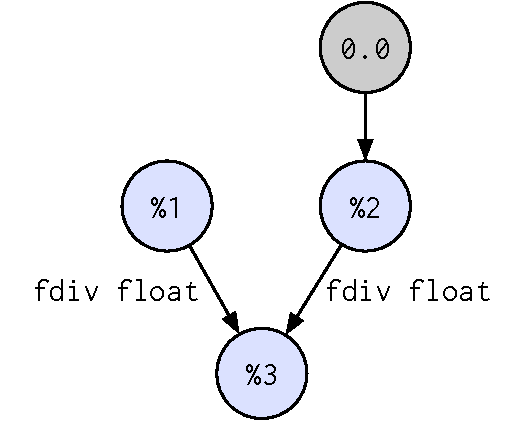
\includegraphics[width=\linewidth]{images/inst2vec.pdf}
      \caption{XFG~\cite{Ben-nun2018}.}
      \label{subfig:inst2vec}
  \end{subfigure}
  \hfill
  \begin{subfigure}{.18\linewidth}
  \vspace{2.4em}
  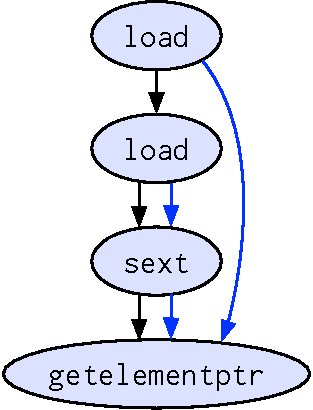
\includegraphics[width=\linewidth]{images/cdfg.pdf}
  \caption{CDFG~\cite{Brauckmann2020}.}
  \label{subfig:cdfg}
  \end{subfigure}
  \caption{%
    Limitations in state-of-the-art learnable code
    representations. In~(\subref{subfig:code2vec}) the model
    over-emphasizes identifier names such that the same algorithm
    produces three different classifications by changing the name of a
    function. The data-flow representation
    of~(\subref{subfig:inst2vec}) does not capture operand order, such
    that non-commutative statements such as division are
    indistinguishable. In~(\subref{subfig:cdfg}) control and data
    relations are captured, but both type information and operand
    order are omitted. Our approach is insensitive to identifier names
    and preserves operand order and type information.%
  }%
\end{figure}


An alternate approach which emphasizes semantics is Neural Code
Comprehension~\cite{Ben-nun2018}, where an encoder uses Contextual
Flow Graphs (XFG) built from LLVM-IR statements to create inputs for
neural networks. The XFG combines partial data- and control-flow to
represent the context of an individual statement. The statements are
then mapped to latent-space representations using their neighbors in
that graph. However, in partially combining DFGs and CFGs, the XFG
representation omits important information such as order of
instruction operands (as shown in Figure~\ref{subfig:inst2vec}), and
the representation fails to capture execution order, critical for many
optimization tasks.

A recent LLVM-IR representation uses Control and Data Flow Graphs
(CDFG)~\cite{Brauckmann2020}. This representation makes the control
and data relations between instructions explicit, but uses only
instruction opcodes to compute latent representations. This omits
information about programs that may be critical for optimization, such
as data types, the presence of variables and constants, and the
ordering of operands, shown in Figure~\ref{subfig:cdfg}.

Each of the three methods of encoding programs as inputs to neural
networks omit information that is vital for compiler analysis. This
hinders the ability of machine learning models to reason about
optimizations and their impact on program behavior. To address these
shortcomings we require an input representation that captures all
parts of a program's semantics that are required for performing such
analyses.


\paragraph{(II) Model Complexity}

The range of core operators in deep learning on code is largely
confined to recurrent units (e.g. RNN, LSTM, GRU) on sequences. This
poses limitations on the representation space of any such network's
outputs. Take, for instance, dominator tree construction. An LSTM
iterating forward over input code will not be able to solve the task
\emph{by definition}, as statements needs to be analyzed backwards
with respect to dependencies. Yet, the neural network only maintains
$\bigo(1)$ memory capacity w.r.t. program length. Iterating in the
opposite direction, in addition to being problem-specialized, would
still not suffice, as dependencies may ``vanish'' in the corresponding
gradients if dependent statements are far away from each other, such
as in the presence of diverging control flow.

One way to increase the algorithmic complexity of the model is by
allowing it to increase the number of code tokens that are processed
simultaneously during inference. This approach, commonly used in
literature by Transformer Networks~\cite{Vaswani2017}, use preceding
tokens (unidirectional encoding) or preceding and subsequent tokens
(bidirectional encoding) to learn \textit{attention matrices}. Such
matrices ``focus'' the network on certain subsets of tokens, skipping
others. However, this approach scales quadratically in memory and
computation with the number of tokens.

Unlike in natural language text, the dependency structure of code is
made explicit during compilation. We can thus employ domain-specific
knowledge to construct the attention matrices in a scalable manner,
using a graph representation of the tokens with dependencies as
edges. A graph representation not only enables meaningful attention
learning, but also facilitates propagating information across the
graph in a manner similar to typical compiler analyses. Within the
same step, a recurrent unit generates $\bigo(1)$ activations, whereas
a graph NN generates $\bigo(|V|)$.

To demonstrate this expressive power, let us consider control-flow
reachability analysis as a learning task. The goal of the model is to
tag statements that are reachable from one or more given tagged
statements. With a sequential LSTM, the model would have to be trained
to memorize nodes along some linear order of the given program. With
an unbounded number of nodes to track and variably-sized regions to
skip, the task becomes infeasible. A message-passing graph neural
network, in contrast, needs only to learn to pass a message forward in
the case of an existing control-flow edge between two nodes,
essentially learning an identity operation over control-flow edges and
zero on others.

In this work, we overcome the above limitations of prior model and
representation approaches, leveraging the graph structure of IR code,
taking path analysis and the semantics of individual statements into
account.
